% LaTeX adaptation of the official Apart Research submission template.
% US Letter, 1-inch margins, Arial 11 pt body, 1.15 line spacing.
\documentclass[11pt,letterpaper]{article}
\usepackage[margin=1in]{geometry}
\usepackage{fontspec}
\IfFontExistsTF{Arial}{\setmainfont{Arial}}{\setmainfont{Liberation Sans}}
\newfontfamily\titleface{TeX Gyre Termes}
\usepackage{setspace}
\setstretch{1.15}
\usepackage{microtype}
\usepackage{graphicx,booktabs,tabularx,array}
\usepackage{amsmath,amssymb}
\usepackage{tikz}
\usetikzlibrary{arrows.meta,positioning}
\usepackage[numbers,sort&compress]{natbib}
\usepackage{titlesec}
\usepackage{enumitem}
\usepackage{xurl}
\usepackage[hidelinks,pdfusetitle]{hyperref}
\hypersetup{pdfauthor={Muhammad Ali Nasir},pdftitle={SwarmCircuit: Checking Agent Handoffs Against Source State}}
\urlstyle{same}
\usepackage{fancyhdr}
\titleformat{\section}{\normalfont\fontsize{20}{23}\selectfont}{\thesection.}{0.5em}{}
\titlespacing*{\section}{0pt}{20pt}{6pt}
\titleformat{\subsection}{\normalfont\bfseries\fontsize{12}{15}\selectfont}{\thesubsection}{0.5em}{}
\titlespacing*{\subsection}{0pt}{10pt}{4pt}
\setlength{\parindent}{0pt}
\setlength{\parskip}{6pt}
\setlength{\emergencystretch}{2em}
\setlist[itemize]{nosep,leftmargin=1.4em,topsep=3pt}
\setlist[enumerate]{nosep,leftmargin=1.6em,topsep=3pt}
\pagestyle{fancy}
\fancyhf{}
\fancyfoot[C]{\small\thepage}
\renewcommand{\headrulewidth}{0pt}
\renewcommand{\footrulewidth}{0pt}
\newcolumntype{L}[1]{>{\raggedright\arraybackslash}p{#1}}
\newcolumntype{Y}{>{\raggedright\arraybackslash}X}
\title{\titleface\bfseries\fontsize{20}{23}\selectfont SwarmCircuit: Checking Agent Handoffs\\Against Source State}
\author{Muhammad Ali Nasir\\[3pt]\small Independent researcher, Islamabad, Pakistan}

\date{Swarm Alignment Hackathon\enspace\textbar\enspace November 9, 2026}

\begin{document}
\maketitle
\vspace{-1em}
\begin{abstract}
An agent's completion message does not establish that its output is supported or that a dependent action remains authorized. We present SwarmCircuit, a small workflow testbed that makes this distinction visible at an agent handoff. A writer produces structured sales claims from a synthetic CSV; a separate reviewer receives the actual draft and source facts. A checker outside the model recomputes the permitted quantities, and a publication step rechecks both those claims and current runtime authority. One repair may use the actual review and check errors. Original outputs, failures and bounded model-call receipts are retained for inspection. In one live case, two model calls completed six SDK tasks, with no repair required and no typed-claim errors. Before sample access was granted, the same run made no model calls and executed no protected steps. Controlled transport tests also exercise a false claim accepted by a reviewer, an invalid repair, cancellation, expired authority and provider failure. These are implementation checks, not estimates of model reliability. The contribution is an inspectable, bounded handoff protocol and working interface, rather than a general security detector. The current evidence does not establish an advantage over existing permission guards or a ready queue, and the two model roles share one provider.
\end{abstract}

\section{Introduction}
Multi-agent work often advances through reports: one worker says that analysis is finished, and another worker uses its output. A readable trace can show that a message arrived while leaving a more important question unanswered: did the claimed work produce a supported result? Permission can also change while a request is in flight. Treating a model's review or a task's recorded completion as sufficient authority risks passing an unsupported claim to the next step.

We study a narrow question: \textit{can a small agent workflow expose the evidence for a handoff and withhold its final artifact when supported claims or current authority fail a check outside the reporting model?} The setting is deliberately modest. The dataset is bundled and synthetic; the model roles have no tools or permission authority. This lets us inspect the handoff mechanism without confusing a synthetic demonstration with a deployment evaluation.

SwarmCircuit adds three concrete elements: the original draft is passed to a reviewer and retained; a deterministic source check gates publication separately from model judgment; and a local interface shows outputs, decisions and model attempts together. A repair receives actual feedback rather than a scripted replacement. The work fits the event's oversight-and-control track \citep{apart2026}. It does not test collusion, hidden communication or large agent populations.

\textbf{Pre-existing work.} The Python SDK, telemetry and control foundations, the original offline demonstration, and a 2,160-trial synthetic study were prepared before the event. They are not presented as new hackathon results. The event-period work makes the workflow understandable and adds the bounded live writer/reviewer handoff, retained evidence, source checks and failure handling described here. The older study and its failed model pilots remain unchanged.

\section{Related Work}
AI control studies evaluate protocols that use oversight to limit an untrusted model's harmful behavior \citep{greenblatt2024}. Our case borrows the separation between a worker and an oversight decision, but does not reproduce that paper's adversarial evaluation. Both model roles here use the same configured provider, and the deterministic CSV check, rather than a trusted model family, supplies the narrow factual reference.

Multi-agent risk extends beyond the behavior of individual models \citep{hammond2025}. The present work examines one handoff boundary; it provides neither a taxonomy nor a measurement of emergent group risk. Human feedback is also an established framework feature: AutoGen, for example, documents a user-proxy path for human input \citep{autogen}. SwarmCircuit's contribution is not the existence of an approval button. It is the inspectable connection between an actual draft, its review, an external source check and a bounded publication decision in this implementation.

\section{Methods}
\subsection{Workflow and trust boundary}
The implementation uses a Python SDK and FastAPI backend with SQLite persistence and a React/Next.js interface. Six SDK tasks cover planning, public notes, sample access, writing, review and publication. Planning and public notes do not require dataset access. The remaining branch waits at cooperative SDK checkpoints for an operator decision. Granting sample access does not clear an existing operator pause; a separate reviewed resume is required.

Figure~\ref{fig:handoff} separates model judgment from the source check. The CSV tool computes five supported quantities: first- and last-quarter revenue, growth between them, the number of quarters and the sum of quarterly customer counts. That last sum is called customer-quarters; it is not a count of unique people. The writer must also include three fixed limitation labels: revenue is not profit, customer-quarters are not unique customers, and four quarters do not establish a forecast.

\begin{figure}[htbp]
\centering
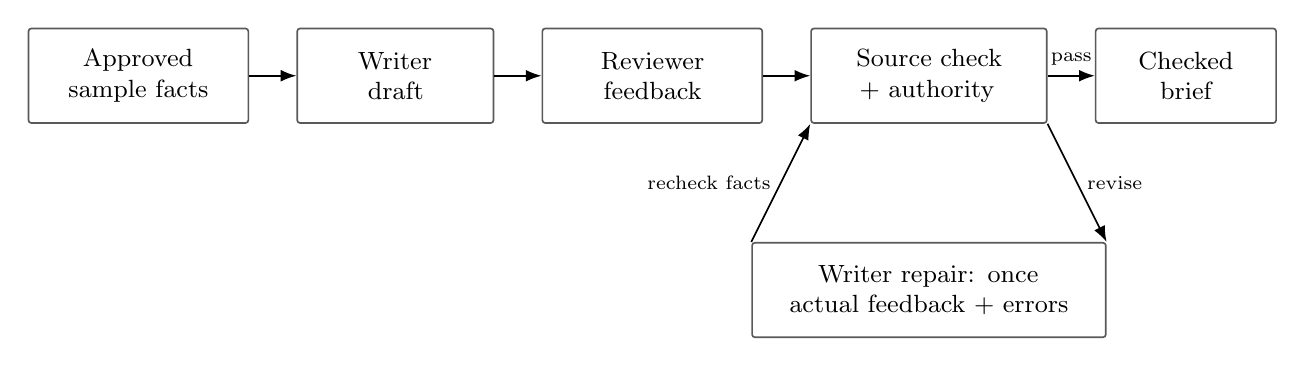
\begin{tikzpicture}[font=\small,>=Latex,box/.style={draw=black!65,rounded corners=1pt,align=center,inner sep=7pt,minimum height=12mm},every path/.style={line width=.6pt}]
\node[box,text width=23mm] (facts) {Approved sample facts};
\node[box,right=6mm of facts,text width=20mm] (writer) {Writer\\draft};
\node[box,right=6mm of writer,text width=23mm] (review) {Reviewer\\feedback};
\node[box,right=6mm of review,text width=25mm] (check) {Source check\\+ authority};
\node[box,right=6mm of check,text width=18mm] (publish) {Checked\\brief};
\draw[->] (facts)--(writer);
\draw[->] (writer)--(review);
\draw[->] (review)--(check);
\draw[->] (check)--node[above,font=\scriptsize]{pass}(publish);
\node[box,below=15mm of check,text width=40mm] (repair) {Writer repair: once\\actual feedback + errors};
\draw[->] (check.south east)--node[right,font=\scriptsize]{revise}(repair.north east);
\draw[->] (repair.north west)--node[left,font=\scriptsize]{recheck facts}(check.south west);
\end{tikzpicture}
\caption{The live handoff, simplified. The reviewer receives the actual draft, recomputed facts and initial check errors. Publication requires current authority and valid typed facts. A failed check can request one repair; a bad repaired candidate is retained without a final brief. The repair receives no second model review.}
\label{fig:handoff}
\end{figure}

The models do not decide permission. Before a provider call and before an output is published, server checks require an active session, approved sample access, an eligible running task, a current runtime owner and control credentials, a valid heartbeat and deadline, and no outstanding queued, dispatched or unknown control request for that task. SDK pause/resume remains cooperative: this is not a general mechanism for stopping arbitrary code. The live HTTP client additionally supports cancellation of its own in-flight request.

\subsection{Claims and publication rule}
The model's output is a strict JSON object. Decimal-valued strings must be finite and numerically equal to independently recomputed source values; count fields are strict integers. Equivalent decimal formatting is accepted. Unknown fields, unsupported quantities and missing or duplicate limitation labels fail validation. Free-form rationale is retained as evidence and is \emph{not} certified as factual prose.

Let $e(d)$ be the source-check errors in draft $d$, and let reviewer output $r$ contain a verdict and a list of issues. The original draft is accepted only when
\[
e(d)=\varnothing\quad\land\quad r.\mathrm{verdict}=\mathrm{accept}\quad\land\quad r.\mathrm{issues}=\varnothing.
\]
Otherwise, one repair receives the original draft, actual review, source facts and check errors. Publication then recomputes the source facts and rejects any remaining typed-claim errors. A successful final brief renders only the supported structured quantities and fixed limitations. It does not promote the model's rationale into checked prose.

\subsection{Model calls and retained evidence}
The recorded live case requested \texttt{DeepSeek-V4-Flash} from the user-configured third-party endpoint \texttt{api.hcnsec.cn}. The response reported the same model name; this is provider metadata, not independent authentication of the underlying model. Temperature was 0.2, with a maximum of 1,100 output tokens per request. The system prompt specifies the JSON schema, treats notes and worker text as data, and grants the model no tools or permission authority. Appendix~\ref{app:reproduce} specifies payloads and reproduction steps.

Each attempt is persisted before network I/O. A durable per-run ceiling permits three attempts: writer, reviewer and at most one repair. There is no automatic retry or offline fallback. The client has a 30-second wall limit, bounded response sizes and cancellation handling. Missing or malformed usage is unknown rather than zero. Draft, review, repair when present, source checks, timestamps and response hashes remain available. These hashes support artifact integrity checks; they are not tamper resistance against an administrator who controls the database.

\subsection{Evaluation design}
We distinguish three kinds of evidence. First, one actual provider execution tests the complete live path. Second, an offline denial run tests that public work survives while protected work remains blocked. Third, injected provider responses test specific acceptance, repair and interruption conditions through the actual SDK/API bridge. They do not add real model samples. Release checks cover client parsing, handoff lifecycle, migrations, API behavior and the web gateway. No comparative model experiment or human-subject study was conducted.

\section{Results}
\subsection{Observed live execution}
The retained live run completed all six tasks using two actual model requests. The original writer draft passed the typed source check; the reviewer accepted it with no issues. No repair was needed. Before access approval, public notes had completed, four tasks were waiting, and both model calls and protected effects were zero. After approval, four protected workflow steps completed. Table~\ref{tab:live} reports the observed quantities, not an estimated error rate.

\begin{table}[htbp]
\centering
\small
\begin{tabularx}{\linewidth}{@{}Y L{56mm}@{}}
\toprule
Observation & Retained value\\
\midrule
Task completion & 6 of 6 SDK tasks\\
Provider attempts & 2 of a maximum of 3\\
Provider-reported input / output tokens & 997 / 304 total\\
Original / final typed-claim errors & 0 / 0\\
Review verdict / issues & Accept / empty list\\
Repair used & No\\
Downloaded artifacts matching stored SHA-256 & 6 of 6\\
\bottomrule
\end{tabularx}
\caption{One actual live case, retained under demo ID \texttt{d449f1a6-1ba2-4f04-aaee-774197881a11}. Usage is reported by the provider. This table does not measure model accuracy across tasks or providers.}
\label{tab:live}
\end{table}

The checked source values were 120,000 and 166,980 sample revenue units in the first and last quarters, 39.15\% growth, four quarters and 1,800 customer-quarters. The independent offline denial case retained the public findings with two of six tasks complete and zero protected effects. These outcomes remained readable after the server restarted. No prices, monetary savings or production effects were inferred from token counts or task states.

\subsection{Controlled failures and release checks}
Table~\ref{tab:failures} summarizes representative injected conditions. In the false-claim test, a reviewer explicitly accepts an incorrect writer value. The source check still requires repair. When the repaired value is also wrong, the draft and failure evidence remain, but no final brief is published. Thus the model's acceptance alone does not determine publication in this implementation. The test establishes the stated branch behavior, not the frequency with which models produce such errors.

\begin{table}[htbp]
\centering
\small
\begin{tabularx}{\linewidth}{@{}L{50mm}Y@{}}
\toprule
Injected condition & Verified implementation behavior\\
\midrule
False writer fact, accepting reviewer & Source mismatch triggers a repair.\\
Invalid repaired candidate & Repair retained; final brief absent.\\
Provider error, timeout or malformed output & Attempt retained; failure without an offline substitute.\\
Cancellation, expiry or authority loss after reply & Output withheld; uncertain attempts remain visible.\\
Three existing attempts & A fourth transport call is refused.\\
\bottomrule
\end{tabularx}
\caption{Controlled transport/API tests. These conditions were injected for verification and were not observed failures in the single successful live execution.}
\label{tab:failures}
\end{table}

The final release checks passed 208 backend tests, 18 frontend unit tests and six live local gateway integration tests; the production web build completed. Thirty-seven focused client/handoff test cases are included in the backend total. These are regression checks, not 208 independent research trials. Tests also cover migration preservation, idempotent mode binding, denial with no provider requests and unknown token usage. A browser regression found and fixed a stale chooser that could incorrectly offer to continue an already-ended walkthrough.

\section{Discussion and Limitations}
The useful result is a concrete distinction between a worker's report and the state required for its handoff. A reader can inspect what the writer produced, what the reviewer saw and why publication was allowed. The checker can reject a supported-schema error even when a reviewer accepts it. The interface also distinguishes completed historical work from connected workers and shows permission decisions separately from operator pauses.

The testbed is intentionally easy to verify: five known quantities and three limitation labels. It does not establish that a model can discover arbitrary factual errors, safely use an open-ended toolset or resist an adversarial collaborator. Same-provider roles can share failure modes. The deterministic checker can be wrong, and malicious modification of source data or server code is outside the tested boundary. A compromised operator or database administrator can alter retained evidence. Cooperative checkpoints do not stop actions that bypass the SDK.

There is one successful model execution, no model-family comparison, no repeated-trial uncertainty estimate and no deployment outcome. We have not shown incremental benefit over permission guards, deduplication or a simple ready queue. The pre-existing synthetic study includes strong simpler baselines and unfavorable graph/telemetry cases; the live case does not overturn them. A next evaluation should hold the task, model and budget fixed while comparing model review alone, source checks and a ready-queue baseline over repeated, independently scored handoffs. It should report withheld correct outputs as well as published incorrect ones.

\section{Conclusion}
SwarmCircuit demonstrates a bounded live handoff whose final artifact depends on source-state checks and current authority, rather than a completion message alone. The actual case and controlled failures make that mechanism inspectable. The evidence supports a working narrow protocol and its implementation checks; broader claims about swarm safety, comparative advantage or human-rights compliance require further evaluation.

\section*{Code and Data}
Source code: \url{https://github.com/al1-nasir/swarm_circuit}. The synthetic dataset and calculation code are in \texttt{demo/fixtures.py}. Retained drafts, reviewer feedback, source checks and model-call receipts are in \texttt{artifacts/live-handoffs-2026-11-08/}. Appendix~\ref{app:reproduce} describes how to run the workflow and verify its outputs. Credentials and runtime databases are excluded from the shared materials.

\clearpage
\bibliographystyle{plainnat}
\bibliography{references}

\clearpage
\appendix
\section{Limitations and Dual-Use / Ethical Considerations}
\label{app:ethics}
\textbf{Human agency and accountability.} The operator sees the scope and reason for a sample decision; denying access preserves public work and prevents protected steps. A recorded permission grant does not silently resume a separately paused task. These design choices support notice and accountable intervention, but they do not establish that a real affected person has an effective appeal or remedy. A production use would need a designated human decision-maker, a way to contest an adverse outcome, retention rules and access controls. Rights to privacy and effective remedy motivate that requirement \citep{udhr1948}; this software is not a legal-compliance assessment.

\textbf{Privacy and minimization.} Model message payloads contain bundled synthetic facts, public explanatory notes and the roles' own draft/feedback. They exclude operator reasons, application/runtime credentials and other workspace content. The configured provider key is used only for HTTPS authentication; it is not exposed to the browser or retained evidence. The optional live start identifies the provider and call limit before any request, and sample access must still be approved. Drafts and reviews are intentionally retained. Using real data would require a retention and deletion policy, a lawful basis for processing, provider review and scoped access. The voluntary NIST AI RMF offers a broader risk-management framework; this case does not implement or certify it as a whole \citep{nist2023}.

\textbf{Dual use.} Better traces can help an operator diagnose a benign team, but can also make harmful multi-agent activity easier to coordinate or debug. Exported traces can reveal task structure, commercial information or a person's activity. A hostile operator might use a polished dashboard to create unwarranted confidence, selectively show successful runs or monitor workers without appropriate consent. We therefore label synthetic data, advisory model reviews, unknown usage and failed outcomes, and exclude credentials from exports. Those measures reduce specific presentation and disclosure risks; they do not prevent misuse of the underlying infrastructure.

\textbf{Scope of assurance.} The verifier checks enumerated fields and limitation labels, not arbitrary rationale, fairness, intent or all downstream effects. A repaired draft receives deterministic checks without another model review. There is no independent trusted-model family, network sandbox, collusion test, external audit, human-subject evaluation or demonstrated deployment benefit. The run cap constrains requests made by this client, not charges caused outside it or the provider's internal behavior. No real company records, production permissions, financial transactions or personal-data decisions were involved in the reported case.

\section{Reproduction and Evidence}
\label{app:reproduce}
\subsection*{Local reproduction}
Install the locked Python environment and Studio dependencies, initialize a private local environment and database, then run the API and interface:
\begin{verbatim}
make bootstrap
make init-local
make db-init
npm --prefix apps/studio ci
make server PORT=18005
# In a second terminal:
SWARM_API_URL=http://127.0.0.1:18005 make studio STUDIO_PORT=3300
\end{verbatim}
Open \url{http://127.0.0.1:3300/demo}. Offline mode makes no model calls. For live mode, privately configure \texttt{SWARM\_MODEL\_BASE\_URL}, \texttt{SWARM\_MODEL\_NAME} and \texttt{SWARM\_MODEL\_API\_KEY} on the server. Review the provider and call ceiling, then sample access. A new live run can incur charges; its wording and usage need not match the retained case.

\subsection*{Prompt and payload contract}
The system instruction requires one schema-matching JSON object, treats worker text as data and gives the model no tools or permission authority. Writer instructions require exact supplied facts and all three limitations. Reviewer instructions require concrete issues for unsupported claims. Payloads contain:
\begin{itemize}
\item Writer: computed CSV facts and bundled public notes.
\item Reviewer: computed facts, the actual writer draft and independent source-check errors.
\item Repair: computed facts, original draft, actual reviewer feedback and source-check errors.
\end{itemize}
Exact prompts and schemas are in \path{demo/agents.py}; transitions in \path{demo/live.py} and \path{demo/service.py}; source data in \path{demo/fixtures.py}, under \path{packages/server/src/swarmcircuit_server/}.

\subsection*{Retained evidence and test commands}
\path{artifacts/live-handoffs-2026-11-08/} contains statuses, six Markdown artifacts, attempt receipts and hash verification. The case began November 7 at 22:17 UTC (November 8 in Pakistan); the third call was unused. November 9 release logs record the checks. Run \texttt{make check}, \texttt{npm --prefix apps/studio run check}, and, against running services, \texttt{npm --prefix apps/studio run test:integration}. These checks require no paid model calls.

\section{LLM Usage Statement}
Codex assisted implementation, debugging, tests, interface copy, evidence checks and report drafting. The live writer and reviewer use the disclosed third-party model. Reported measurements come from retained artifacts, receipts and release logs. The author is responsible for the event-work disclosure, final review and submitted materials. AI assistance does not constitute independent scientific review.

\end{document}
